\chapter{Introduction}
\label{cha:Introduction}

\section{Motivation}
\subsection{Path planning in robotics}
In robotics the path planning of a robot can be programmed as a fixed list of movements to be executed. This has multiple drawbacks as for every change in the enviroment the robot needs to manually be reprogrammed.\\
But what if we equip this robot with a camera that detects the shape of objects in the robots enviroment. This would give us a set of objects at certain position, a robot arm in a starting position and a target where the robots endeffector needs to work. If we would be able to solve this puzzle, we could direct the robot in a different way each time without the actual need to access its software.


\subsection{Geometric riddles in gaming}
Solving geometric riddles is a amazingly fun task for a human. This is the reason many games simply consists of such riddles ranking from easy to hard in difficulty. But even the easiest riddle for a human proposes a big challenge for a simple algorithm that searches trough the possible ways of solving it. Even more complicated is the generation of such riddles. Even for the human brain this task can be exceedingly stressful.\\
 Now, if there would be a possibility to check if such a riddle has a solution, there would be the option to generate them randomly and check for feasability. This would release the developers of the need to manually create each riddle. Also the consumers, in this case the players, would have a never ending stream of new and different riddles to solve.



\section{Idea}
As the representation behind these two cases is the same, for simplification purposes we break the riddles down into two dimensional object displacement problems. The following riddles shall provide simple example of the problem:\\

\begin{figure}[h]
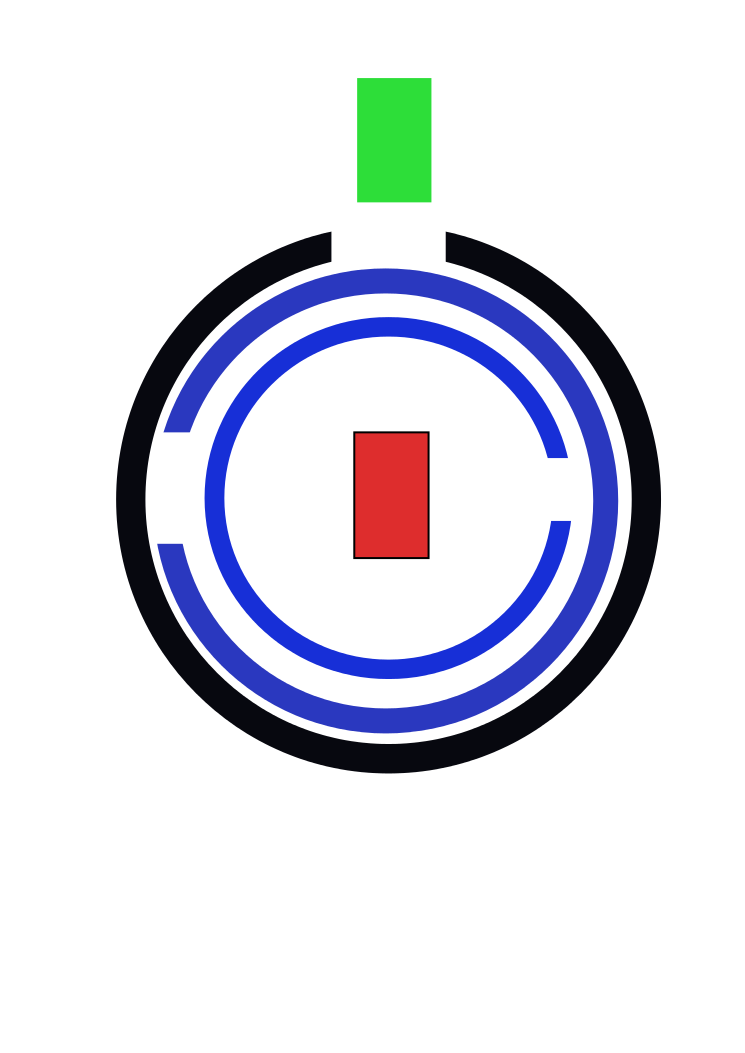
\includegraphics[scale=0.1]{circleRiddle.png}
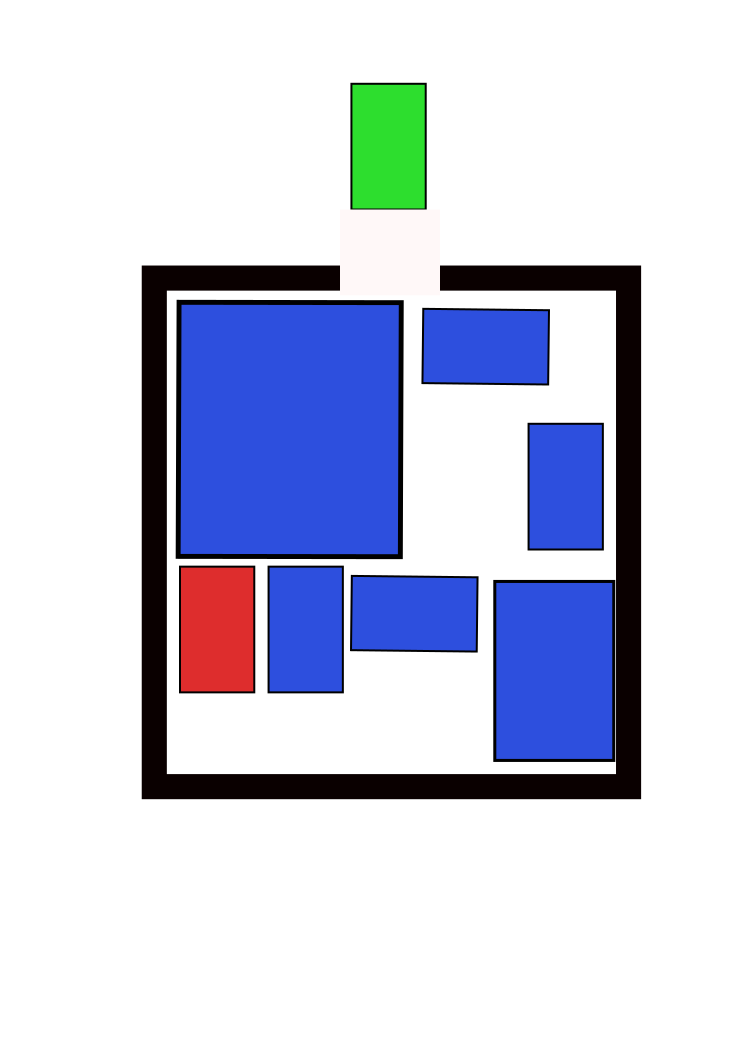
\includegraphics[scale=0.1]{boxRiddle.png}
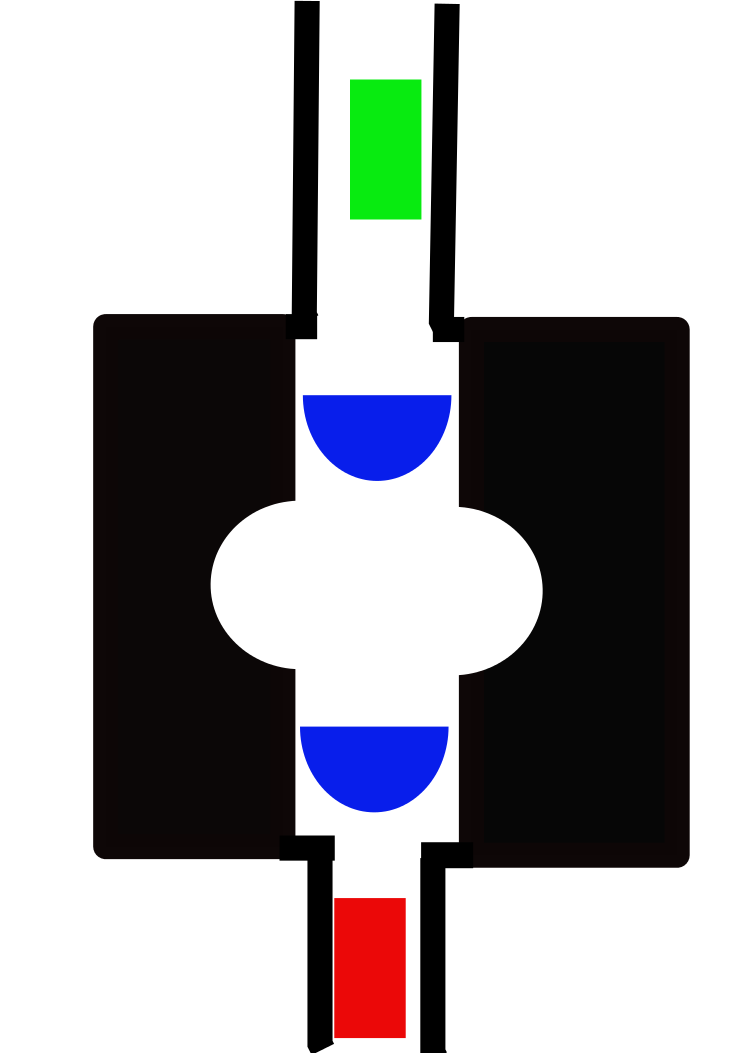
\includegraphics[scale=0.1]{mixedRiddle.png}
\caption{riddle 1 with circles , riddle 2 with boxes , riddle 3 with 2 half-circles}
\end{figure}

The riddle is solved, if the red box matches the green one. Blue objects are movable and black ones are stationary. The stationary ones will be referred to as rims hereafter.\\
As a human the way to solve those is quite obvious. The first riddle is solved by rotating the blue objects, the second through translation. The third needs both ways to be solved.\\
If we want to solve this with an algorithm, we would need to consider each objects collsision with the other objects and the rim. Also we would need to find a way to express the current configuration consisting of position (x,y) and rotation ($\phi$) and the direction the main object needs to take. A simple idea would be to 
\begin{enumerate}
\item generate all valid configurations per object in regard to the stationary obstacles as a configuration space
\item Create one collision space per object for collision with every other object. 
\item Substract the collision space from the configuration space to get valid space in regard to all obstacles for one object.
\item Divide the space in cells and locate the valid ones.
\item Build a graph out of this starting position by adapting the space after each step.
\item Search in that graph to get path from start to target point.
\end{enumerate}

The target point would then be a simple configuration vector holding each position of each object. A user defined distance function beetween start and target point in that space can then be used as heuristic in the graph search ( e.g. $h(start,target) = || ( x_{start} -  x_{target} , y_{start} - y_{target} ) ||$ ).
